
\documentclass[tikz, border=10mm]{standalone}
\usepackage{xcolor}
\usepackage{tikz}
\usetikzlibrary{positioning, calc, backgrounds, quotes, arrows.meta}

% Inline definition of styles to avoid dependency hell for legend
\definecolor{ConvColor}{rgb}{0.98,0.81,0.69}
\definecolor{PoolColor}{rgb}{0.8,0.33,0.33}
\definecolor{UnpoolColor}{rgb}{0.6,0.7,0.9}
\definecolor{FcColor}{rgb}{0.6,0.2,0.8}
\definecolor{ResBlockColor}{rgb}{0.85,0.92,1.0}

% 2D Styles
\tikzset{
    layer/.style={
        rectangle,
        rounded corners=1mm,
        minimum height=2.0em,
        minimum width=3.0em,
        align=center,
        draw=black!80,
        thick
    },
    conv/.style={layer, fill=ConvColor},
    pool/.style={layer, fill=PoolColor},
    up/.style={layer, fill=UnpoolColor},
    res/.style={layer, fill=ResBlockColor},
    fc/.style={layer, fill=FcColor},
    skip/.style={->, dashed, draw=blue!60, thick}
}

% Simple 3D Box approximation for Legend (to avoid Box.sty compilation issues)
\tikzset{
    box3d/.style={
        shape=rectangle,
        draw=black!50,
        fill=#1,
        minimum width=1cm,
        minimum height=1.5cm,
        append after command={
            \pgfextra{
                \draw[fill=#1!80!black, draw=black!50] (\tikzlastnode.north east) -- ++(0.3,0.3) -- ++(-1,0) -- (\tikzlastnode.north west) -- cycle;
                \draw[fill=#1!60!black, draw=black!50] (\tikzlastnode.north east) -- ++(0.3,0.3) -- ++(0,-1.5) -- (\tikzlastnode.south east) -- cycle;
            }
        }
    }
}

\begin{document}
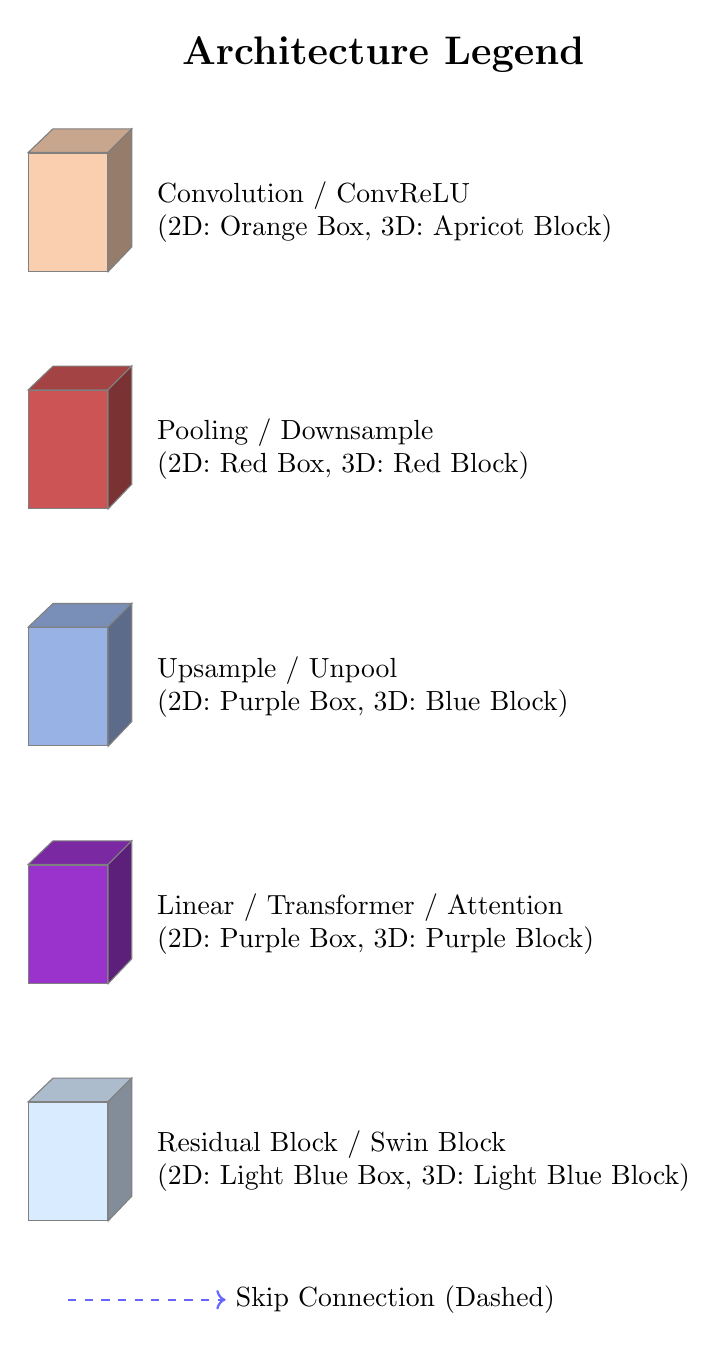
\begin{tikzpicture}[node distance=0.8cm, every node/.style={transform shape}]

% Title
\node[font=\Large\bfseries] at (4, 7) {Architecture Legend};

% --- 2D / 3D Unified Colors ---
% Since we use consistent colors, we can show one legend for both

\coordinate (start) at (0, 5);

% Conv
\node[box3d=ConvColor] (l_conv) at (start) {};
\node[right=0.5cm of l_conv, align=left] {Convolution / ConvReLU\\(2D: Orange Box, 3D: Apricot Block)};

% Pool
\node[box3d=PoolColor, below=1.5cm of l_conv] (l_pool) {};
\node[right=0.5cm of l_pool, align=left] {Pooling / Downsample\\(2D: Red Box, 3D: Red Block)};

% Up
\node[box3d=UnpoolColor, below=1.5cm of l_pool] (l_up) {};
\node[right=0.5cm of l_up, align=left] {Upsample / Unpool\\(2D: Purple Box, 3D: Blue Block)};

% FC
\node[box3d=FcColor, below=1.5cm of l_up] (l_fc) {};
\node[right=0.5cm of l_fc, align=left] {Linear / Transformer / Attention\\(2D: Purple Box, 3D: Purple Block)};

% Res
\node[box3d=ResBlockColor, below=1.5cm of l_fc] (l_res) {};
\node[right=0.5cm of l_res, align=left] {Residual Block / Swin Block\\(2D: Light Blue Box, 3D: Light Blue Block)};

% Skip
\draw[skip] ($(l_res.south) + (0, -1)$) -- ++(2, 0) node[right] {Skip Connection (Dashed)};

\end{tikzpicture}
\end{document}
